\documentclass[10pt,journal,letterpaper]{IEEEtran}
\usepackage{xr-hyper}
% SPS manuscript guidelines specify double-column 10pt and one-inch margins.
\usepackage[margin=1in]{geometry}
\usepackage{cite}
\usepackage{graphicx}
\usepackage{amsmath,amssymb,amsfonts,mathtools}
\usepackage{booktabs,multirow,array}
\usepackage{xspace}
\usepackage{microtype}
\usepackage{needspace}
\usepackage{placeins}
\raggedbottom
\usepackage[hidelinks]{hyperref}
\newcommand{\ours}{DEDBSR\xspace}
\newcommand{\lr}{\mathrm{LR}}
\newcommand{\hr}{\mathrm{HR}}
\newcommand{\teacher}{\mathrm{T}}
\newcommand{\student}{\mathrm{S}}
\newcommand{\best}[1]{\textbf{#1}}
\newcommand{\second}[1]{\underline{#1}}
\hyphenation{super-resolution re-con-struc-tion}
\hyphenation{trans-form deg-ra-da-tion con-trast-ive spa-tial}

\externaldocument[main-]{main}
\title{Supplementary Material for DEDBSR: Deep Ensemble Distillation for Blind Image Super-Resolution}
% Author names/order/affiliations were not supplied in the source draft.
% Fill with verified author information before submission.
\author{}

\markboth{DEDBSR: Supplementary Material}{DEDBSR}
\begin{document}
\maketitle
\setcounter{figure}{4}
\setcounter{table}{7}
\setcounter{equation}{15}
\setcounter{section}{6}


\section{Implementation and Training}
\label{sec:supp_impl}
\subsection{Data and Architecture}
We train on 3,450 DF2K images (800 DIV2K and 2,650 Flickr2K). Flipped and rotated $256\times256$ HR crops yield $64\times64$ LR inputs. The primary setting applies $21\times21$ isotropic Gaussian blur, bicubic $\times4$ downsampling, and LR rounding/clamping to $[0,255]$, followed by normalization. No noise is added.

Teachers sample $\sigma\sim\mathcal U[0.2,4]$. Student sampling is 75\% uniform and 25\% an equal mixture centered at $1.2,2.4,3.6$, with standard deviation 0.15 and clipping to $[0.2,4]$. The main test widths therefore receive increased training density; intermediate widths within this interval are not out of distribution.

The teacher concatenates RGB LR with a broadcast 15-dimensional kernel PCA code (18 channels, no noise-level channel); the student uses RGB alone. Initial conditions have 64 channel entries and eight spatial channels.

Each of eight groups contains ten modulated blocks, a ConvNeXt block, and a convolution. Group-specific updates act on conditions before each group. The spatial path uses a standard $5\times5$ convolution; the subsequent ConvNeXt block includes a $7\times7$ depthwise convolution.

The $64\!\rightarrow\!16\!\rightarrow\!8$ router reads the initial channel condition. Its last layer and the residual fusion convolution start at zero; the fusion-gate logit starts at $-1.5$.

\subsection{Checkpoint Assignments}
Main Table~\ref{main-tab:main} gives the original benchmark. The additional CdCL comparison and transfer controls use the student model initialized from the recorded teacher checkpoint. Both indices count cumulative training epochs: the designated student model follows the recorded warm-up and reconstruction stages; the scheduled endpoint is not used in this comparison. Motivation images use a teacher checkpoint; the larger prefix probe uses a separate teacher checkpoint; the teacher/student valley probe uses recorded teacher and student models.

Figure~\ref{main-fig:qualitative} reproduces the img092 comparison in the upper panel and the original img093 comparison in the lower panel, preserving their existing crops, method labels, and arrangement.

\subsection{Teacher Objective}
Four patches from each image share a sampled kernel. Let $q_{b,i}$ and $k_{b,j}$ be L2-normalized 128-dimensional query and momentum-key projections. For $P=4$ patches, all ordered within-image pairs $i\ne j$ are positives:
\begin{equation}
\begin{split}
\mathcal L_{\rm con}={}&-\frac{1}{BP(P-1)}\sum_{b,i}\sum_{j\ne i}
\log\frac{e^{q_{b,i}^{\mathsf T}k_{b,j}/\tau}}
{e^{q_{b,i}^{\mathsf T}k_{b,j}/\tau}+Z_{b,i}},\\
Z_{b,i}={}&\sum_{v\in\mathcal Q}e^{q_{b,i}^{\mathsf T}v/\tau}.
\end{split}
\label{eq:supp_con}
\end{equation}
The FIFO queue contains 8,192 keys, $\tau=0.07$, and key-encoder momentum is 0.999. Only the first-patch key is enqueued. Queue entries are not filtered by degradation distance; the PCA code conditions the encoder without reweighting pairs. The first 100 epochs use $\mathcal L_{\rm con}$ alone. During the following 600 epochs, first-patch RGB reconstruction is added with unit weight:
\begin{equation}
\mathcal L_T=\mathcal L_{\rm con}+\frac1B\sum_b
\operatorname{mean}|255\hat{\mathbf x}_{T,b,1}-\mathbf x^{255}_{b,1}|.
\label{eq:supp_teacher}
\end{equation}
The target $\mathbf x^{255}$ lies in $[0,255]$. The student inherits the specified teacher checkpoint rather than the scheduled endpoint.

\subsection{Student Training}
Condition alignment acts only on initial states. We use MSE on the spatial state to preserve its amplitude, MAE on the channel state to reduce sensitivity to outliers, and KL on the normalized channel distribution to retain relative assignments:
\begin{equation}
\begin{split}
\mathcal L_{\rm cond}={}&\operatorname{MSE}(\mathbf s_S,\mathbf s_T)
+D_{\rm KL}(p_T\Vert p_S)\\
&+0.1\operatorname{MAE}(\mathbf c_S,\mathbf c_T),\quad
p=\operatorname{softmax}(\mathbf c/0.15).
\end{split}
\label{eq:supp_student_cond}
\end{equation}
In the main paper's condition-alignment objective, $\lambda_c=0.1$ and $T=0.15$; the equation above instantiates those coefficients. MSE and MAE are element means; KL sums over channels and averages over samples without an extra temperature-squared factor. Teacher targets are detached. Later conditions, increments, and routes receive no direct alignment loss. Warm-up minimizes $\mathcal L_{\rm cond}$; the joint objective is
\begin{equation}
\begin{aligned}
\mathcal L_S&=\mathcal L_{\rm GT}+\mathcal L_{\rm cond},\\
\mathcal L_{\rm GT}&=\mathcal L_{\rm rec}+\lambda_o(t)\mathcal L_{\rm out}.
\end{aligned}
\label{eq:supp_student}
\end{equation}
where $\mathcal L_{\rm rec}$ is the GT reconstruction term and the GT-guided composite $\mathcal L_{\rm GT}$ has the same meaning as in the main paper. Here $\lambda_{\rm rec}=1$ and $\lambda_o(t)$ corresponds to $\lambda_{\rm out}(t)$ in the main paper. Reconstruction and output-imitation losses use mean absolute RGB error after multiplying predictions by 255. For a detached patch gate $m_b=\mathbb1[\ell_{T,b}<\ell_{S,b}]$, device $d$ computes
\begin{equation}
\mathcal L_{\rm out}=
\frac{\sum_{b\in\mathcal B_d}m_b\operatorname{mean}|255\hat{\mathbf x}_{S,b}-255\hat{\mathbf x}_{T,b}|}
{\max(1,\sum_{b\in\mathcal B_d}m_b)}.
\label{eq:supp_output}
\end{equation}
Distributed training averages device-local losses; it does not normalize by a global count of accepted patches. At SR epoch $t\ge1$,
\begin{equation}
\lambda_o(t)=0.05+0.075\left[1+\cos\frac{\pi\min(t,300)}{300}\right].
\label{eq:supp_lambda}
\end{equation}
GT acts on every joint-stage patch, but not during condition warm-up. Closing the output gate leaves condition alignment and inherited initialization intact. Thus it removes direct output imitation on teacher-worse patches, without guaranteeing freedom from all teacher-induced errors. In the frozen 400-patch risk probe, the rule closed all 138 teacher-worse patches and opened all 262 teacher-better patches. This verifies the intended risk partition only; it does not imply a positive post-training gain.

Student training uses four GPUs, 16 samples per GPU, Adam $(0.9,0.99)$, gradient clipping at 1.0, and EMA decay 0.999. The SR learning rate warms up for five epochs to $2\times10^{-4}$, then decays to $10^{-6}$ over 600 SR epochs. Table~\ref{tab:supp_schedule} specifies the historical controls in main Table~\ref{main-tab:controls} at the designated student model; their full metrics appear in Table~\ref{tab:supp_transfer_complete}.

Full and F1 have matching recorded teacher initialization, different-budget batch-64 training, and 100 condition-warm-up plus 500 reconstruction epochs. F1 removes direct output KD and exceeds Full by 0.0094~dB in the twelve-condition mean; each wins six conditions. This historical comparison does not isolate the gate, because removing output KD also removes all direct teacher-output supervision.

GT-only/F2/F4 instead have 600 reconstruction-stage epochs. F3 uses condition alignment alone throughout, with no reconstruction stage. F4 disables the GT-relative gate and uses only output KD, without GT reconstruction or condition alignment. F5 freezes the restoration network, including its upsampler, and updates the LR encoder and condition projections. These distinctions prevent pooling all rows into a single matched loss comparison.

The additional Gate-on, Gate-off, and No-output-KD diagnostics start from the same student checkpoint and receive the same 3 recovery epochs and 8,409 updates. Their twelve-condition equal-mean PSNRs are 28.5203, 28.5280, and 28.5170~dB, respectively: Gate-on minus Gate-off is $-0.0077$~dB, and Gate-on minus No-output-KD is $+0.0032$~dB. These means first average images within each dataset--width condition and then weight all twelve conditions equally, as in the other aggregate tables. Pooling the 657 image--width observations instead gives 27.0365, 27.0469, and 27.0384~dB; the corresponding Gate-on differences are $-0.0104$ and $-0.0019$~dB. Both aggregations are reported here to distinguish their weighting conventions.

Each branch also evaluates the separate 100-image Urban100 stress condition at $\sigma=4.6$, where Gate-on minus Gate-off/No-output-KD is $-0.1327/-0.0567$~dB.

The fixed teacher-worse subset is defined at initialization, before any recovery outcome is observed. On its 138 patches, Gate-on minus Gate-off is $-0.0694$~dB, with 95\% fixed-patch bootstrap interval $[-0.0824,-0.0561]$~dB. Over all 400 fixed patches, the difference is $-0.0704$~dB with interval $[-0.0840,-0.0571]$; Gate-on minus No-output-KD is $-0.0036$~dB with interval $[-0.0162,+0.0092]$.

These intervals use 10,000 resamples and measure patch-sampling uncertainty, not training-run variability. An additional output-guidance isolation removes condition KD while retaining GT reconstruction and output KD; Gate-on minus Gate-off is $-0.0474$~dB over all 400 patches, with 95\% interval $[-0.0609,-0.0349]$~dB. This isolation differs from historical F4, which has no GT loss. The finite recovery results separate the correctness of the risk-partition rule from its training effect and do not establish a positive causal accuracy gain for the gate.

\begin{table}[t]
\caption{Historical stage lengths for the recorded training stages; all use global batch 64. Stage counts are not equalized reconstruction budgets.}
\label{tab:supp_schedule}
\centering\scriptsize
\setlength{\tabcolsep}{3pt}
\begin{tabular}{lrl}
\toprule
Configuration & \shortstack{Condition\\warm-up} & \shortstack[l]{Following objective\\and epochs}\\
\midrule
Full / F1 / F5 & 100 & Reconstruction / 500\\
GT-only, scratch/initialized & 0 & GT reconstruction / 600\\
F2: no condition KD & 0 & GT + output KD / 600\\
F3: condition only & 100 & Condition alignment / 500\\
F4: output KD only, no GT & 0 & Output KD only / 600\\
\bottomrule
\end{tabular}
\end{table}

\begin{table*}[t]
\caption{Historical student-checkpoint transfer controls: complete PSNR (dB) and available SSIM. Columns are blur widths within each dataset. Stage differences in Table~\ref{tab:supp_schedule} apply; these values are not isolated, equal-budget loss effects. GT-only denotes initialized reconstruction.}
\label{tab:supp_transfer_complete}
\centering\footnotesize
\setlength{\tabcolsep}{3pt}
\begin{tabular}{l|rrr|rrr|rrr|rrr}
\toprule
 & \multicolumn{3}{c|}{Set5} & \multicolumn{3}{c|}{Set14} & \multicolumn{3}{c|}{B100} & \multicolumn{3}{c}{Urban100}\\
Model & 1.2&2.4&3.6&1.2&2.4&3.6&1.2&2.4&3.6&1.2&2.4&3.6\\
\midrule
\multicolumn{13}{l}{PSNR}\\
Full &32.496&32.270&31.096&28.945&28.740&27.689&27.809&27.716&27.070&26.657&26.326&25.341\\
GT-only &32.447&32.209&31.044&28.915&28.745&27.718&27.804&27.709&27.068&26.649&26.329&25.409\\
F1 &32.509&32.248&31.080&28.933&28.734&27.768&27.807&27.712&27.074&26.659&26.335&25.409\\
F2 &32.475&32.244&31.090&28.926&28.744&27.720&27.806&27.711&27.076&26.640&26.323&25.422\\
F3 &32.271&32.155&30.453&28.927&28.396&26.633&27.791&27.595&26.768&26.008&26.044&23.592\\
F4 &32.453&32.189&31.064&28.961&28.757&27.634&27.816&27.719&27.073&26.674&26.339&25.413\\
F5 &32.224&32.103&30.689&28.936&28.762&27.232&27.789&27.649&26.949&26.359&26.247&24.149\\
\midrule
\multicolumn{13}{l}{SSIM}\\
Full &.8982&.8929&.8694&.7875&.7788&.7407&.7415&.7347&.7006&.8014&.7887&.7487\\
F1 &.8982&.8927&.8694&.7871&.7786&.7424&.7413&.7346&.7014&.8015&.7888&.7515\\
F2 &.8981&.8930&.8687&.7871&.7793&.7409&.7416&.7349&.7017&.8013&.7891&.7519\\
F3 &.8976&.8899&.8559&.7902&.7717&.7049&.7444&.7364&.6889&.7996&.7894&.6778\\
F4 &.8980&.8929&.8679&.7880&.7797&.7390&.7418&.7354&.7008&.8018&.7897&.7503\\
F5 &.8968&.8928&.8636&.7898&.7802&.7246&.7436&.7367&.6966&.8032&.7894&.7037\\
\bottomrule
\end{tabular}
\end{table*}


\section{Uniform-Weight Evaluation}
\label{sec:supp_uniform_training}
Table~\ref{tab:supp_uniform_training} gives the complete corrected Full/uniform replay. Both models execute all groups and retain the residual branch and fusion projection; the uniform model replaces the route by $1/8$. Initialization, data, different-budget batch-64 schedule, and evaluation device are matched. Stored architecture size is retained, but the uniform route does not use the router's learned outputs. This is not a learned-global-static or an active-capacity-matched no-ensemble control.

PSNR/SSIM use quantized luminance, a four-pixel border crop, and the same LR-generation pipeline. Dataset--width scores average image-level metrics; the overall mean weights the twelve conditions equally. The corrected mean PSNRs are Full/uniform 28.513/28.519 at the designated student model and 28.516/28.519 at the later evaluation state. This replay is separate from the original benchmark aggregates. One recovered run per variant supports near parity, without a run-level variance claim; the two evaluation states are not independent repetitions.

\begin{table*}[t]
\caption{Complete corrected replay: PSNR (dB) and SSIM for four datasets and three blur widths. Full and the separately trained uniform model retain the residual branch. Each variant supplies one recovered training run; the the two evaluation states do not constitute independent repetitions.}
\centering\footnotesize
\setlength{\tabcolsep}{2.2pt}
\begin{tabular}{lc|ccc|ccc|ccc|ccc}
\toprule
Ensemble & Run & \multicolumn{3}{c|}{Set5} & \multicolumn{3}{c|}{Set14} & \multicolumn{3}{c|}{B100} & \multicolumn{3}{c}{Urban100}\\
& &1.2&2.4&3.6&1.2&2.4&3.6&1.2&2.4&3.6&1.2&2.4&3.6\\
\midrule
\multicolumn{14}{l}{PSNR}\\
Input-dependent & A & 32.493 & 32.276 & 31.095 & 28.945 & 28.739 & 27.686 & 27.809 & 27.716 & 27.070 & 26.657 & 26.326 & 25.342\\
Uniform, retrained & A & 32.520 & 32.282 & 31.113 & 28.935 & 28.723 & 27.706 & 27.815 & 27.713 & 27.073 & 26.648 & 26.311 & 25.383\\
Input-dependent & B & 32.508 & 32.276 & 31.104 & 28.940 & 28.736 & 27.707 & 27.808 & 27.713 & 27.072 & 26.655 & 26.328 & 25.347\\
Uniform, retrained & B & 32.510 & 32.259 & 31.108 & 28.937 & 28.731 & 27.730 & 27.812 & 27.709 & 27.074 & 26.654 & 26.318 & 25.392\\
\midrule
\multicolumn{14}{l}{SSIM}\\
Input-dependent & A & 0.8982 & 0.8930 & 0.8693 & 0.7875 & 0.7788 & 0.7407 & 0.7415 & 0.7347 & 0.7006 & 0.8014 & 0.7887 & 0.7487\\
Uniform, retrained & A & 0.8984 & 0.8931 & 0.8699 & 0.7870 & 0.7784 & 0.7407 & 0.7412 & 0.7346 & 0.7009 & 0.8010 & 0.7885 & 0.7504\\
Input-dependent & B & 0.8983 & 0.8930 & 0.8697 & 0.7873 & 0.7787 & 0.7411 & 0.7414 & 0.7347 & 0.7009 & 0.8014 & 0.7887 & 0.7488\\
Uniform, retrained & B & 0.8983 & 0.8929 & 0.8698 & 0.7872 & 0.7786 & 0.7413 & 0.7414 & 0.7348 & 0.7012 & 0.8012 & 0.7888 & 0.7509\\
\bottomrule
\end{tabular}
\label{tab:supp_uniform_training}
\end{table*}


\section{Condition and Depth Diagnostics}
\label{sec:supp_teacher}
\subsection{Condition Paths}
Standard recurrent teachers A and B are independently trained eight-group, ten-block instances using batch 64 and the same recorded 100+600-epoch recipe; each is evaluated with its own PCA. Their tensors and PCA differ, although both configurations record seed 1. The alternative-budget teacher uses 44,850 training samples per epoch versus 193,200 for the standard recipe and follows a different update budget. These records are neither different-seed statistics nor equal-budget replicas and are not pooled.

One-shot bypasses condition updates; nonrecurrent applies each group's distinct update to the initial state; shared recursively reuses the first group's module. Other components remain fixed. At $\sigma=1.2,2.4,3.6$, all three interventions lose on every Urban100 image for standard teachers A and B. Table~\ref{tab:supp_condition_ci} gives nonrecurrent intervals. The alternative-budget teacher's nonrecurrent penalties are 2.391/2.849/0.088~dB; the last has interval $[0.034,0.139]$ and 80/100 recurrent wins. 

\begin{table}[!t]
\caption{Fixed-teacher interventions on 100 paired Urban100 images per width, without retraining. The two rows are independently trained instances of the same standard recurrent teacher (batch 64, eight groups, ten blocks); they test reproducibility of the recurrence intervention, not hardware effects. $\Delta$ is intervention minus Full. Only widths within training support are shown.}
\label{tab:condition_repeats}
\centering\scriptsize
\setlength{\tabcolsep}{2.5pt}
\resizebox{\columnwidth}{!}{%
\begin{tabular}{llrrrr}
\toprule
Teacher instance & $\sigma$ & Full & $\Delta$ Nonrec. & $\Delta$ One-shot & $\Delta$ Shared\\
\midrule
Standard recurrent teacher A & 1.2 & 26.738 & $-5.136$ & $-4.469$ & $-3.130$\\
Standard recurrent teacher A & 2.4 & 25.346 & $-3.354$ & $-3.183$ & $-2.471$\\
Standard recurrent teacher A & 3.6 & 25.428 & $-3.651$ & $-3.437$ & $-3.647$\\
Standard recurrent teacher B & 1.2 & 26.692 & $-5.255$ & $-5.395$ & $-4.115$\\
Standard recurrent teacher B & 2.4 & 25.421 & $-4.113$ & $-3.893$ & $-3.679$\\
Standard recurrent teacher B & 3.6 & 25.470 & $-4.537$ & $-4.112$ & $-4.586$\\
\bottomrule
\end{tabular}}
\end{table}


\begin{table}[t]
\caption{Fixed-teacher interventions: $\Delta$PSNR (variant minus recurrent), with paired-image 95\% bootstrap intervals. Standard A/B are independent same-recipe teachers; N/O/S denote nonrecurrent/one-shot/shared. Every row contains 100 Urban100 images.}
\label{tab:supp_condition_ci}
\centering\footnotesize
\setlength{\tabcolsep}{3.0pt}
\begin{tabular}{cccrr}
\toprule
Teacher & $\sigma$ & Path & $\Delta$PSNR & 95\% interval\\
\midrule
Standard A & 1.2 & N & $-5.136$ & $[-5.634,-4.664]$\\
Standard A & 2.4 & N & $-3.354$ & $[-3.672,-3.053]$\\
Standard A & 3.6 & N & $-3.651$ & $[-4.045,-3.281]$\\
Standard B & 1.2 & N & $-5.255$ & $[-5.724,-4.808]$\\
Standard B & 2.4 & N & $-4.113$ & $[-4.468,-3.772]$\\
Standard B & 3.6 & N & $-4.537$ & $[-4.979,-4.119]$\\
\midrule
Standard A & 4.6 & N & $+0.543$ & $[+0.486,+0.599]$\\
Standard A & 4.6 & O & $+0.394$ & $[+0.342,+0.448]$\\
Standard A & 4.6 & S & $+0.479$ & $[+0.413,+0.552]$\\
\bottomrule
\end{tabular}
\end{table}


The expanded evaluation adds six widths: $\sigma=0.8$, $1.6$, $2.0$, $2.8$, $3.2$, and $4.0$. Primary-width results use the identical checkpoints. Its 6,000 image--width--variant records cover standard teachers A/B and the alternative-budget teacher, ten widths, two paths, and 100 Urban100 images. Table~\ref{tab:teacher_width_summary} summarizes width groups; Table~\ref{tab:supp_width_complete} preserves each additional width. Standard teacher A has one exception at $\sigma=2.8$; the alternative-budget teacher has three at $\sigma=3.2$. These widths lie inside training support.

\begin{table}[!t]
\caption{Nonrecurrent minus Full PSNR (dB). Primary: $\sigma\in\{1.2,2.4,3.6\}$; additional: $\{0.8,1.6,2.0,2.8,3.2,4.0\}$. Intervals cluster 100 images across widths. Standard teachers A and B share the same recurrent architecture and training recipe; the alternative-budget teacher changes the update budget.}
\label{tab:teacher_width_summary}
\centering\scriptsize
\setlength{\tabcolsep}{3pt}
\resizebox{\columnwidth}{!}{%
\begin{tabular}{lrr}
\toprule
Teacher instance & Primary (3) & Additional (6), 95\% CI\\
\midrule
Standard recurrent teacher A & $-4.047$ & $-3.916\;[-4.300,-3.559]$\\
Standard recurrent teacher B & $-4.635$ & $-4.489\;[-4.887,-4.108]$\\
Alternative-budget teacher & $-1.776$ & $-1.926\;[-2.170,-1.706]$\\
\bottomrule
\end{tabular}}
\end{table}


\begin{table*}[t]
\caption{Complete added-width and stress diagnostics on 100 Urban100 images. Each cell gives nonrecurrent minus recurrent PSNR (dB), its paired-image 95\% interval, and recurrent/nonrecurrent win counts. Standard teachers A/B share the recorded recipe; the alternative-budget teacher changes the update budget. Widths through 4.0 lie inside training support; 4.6 is a predeclared stress test.}
\label{tab:supp_width_complete}
\centering\footnotesize
\setlength{\tabcolsep}{3pt}
\renewcommand{\arraystretch}{1.05}
\begin{tabular*}{\textwidth}{@{\extracolsep{\fill}}crrr@{}}
\toprule
$\sigma$ & Standard A & Standard B & Different-budget\\
\midrule
0.8 & $-5.233\;[-5.732,-4.754];\;100/0$ & $-5.118\;[-5.594,-4.656];\;100/0$ & $-2.360\;[-2.657,-2.086];\;100/0$\\
1.6 & $-4.984\;[-5.482,-4.512];\;100/0$ & $-5.234\;[-5.700,-4.798];\;100/0$ & $-2.726\;[-3.051,-2.420];\;100/0$\\
2.0 & $-4.451\;[-4.883,-4.039];\;100/0$ & $-4.990\;[-5.437,-4.564];\;100/0$ & $-2.931\;[-3.276,-2.613];\;100/0$\\
2.8 & $-2.391\;[-2.659,-2.141];\;99/1$ & $-3.643\;[-3.965,-3.330];\;100/0$ & $-2.367\;[-2.674,-2.080];\;100/0$\\
3.2 & $-2.949\;[-3.258,-2.663];\;100/0$ & $-3.583\;[-3.921,-3.271];\;100/0$ & $-0.725\;[-0.879,-0.588];\;97/3$\\
4.0 & $-3.488\;[-3.878,-3.132];\;100/0$ & $-4.363\;[-4.779,-3.968];\;100/0$ & $-0.445\;[-0.494,-0.399];\;100/0$\\
\midrule
4.6 & $+0.543\;[+0.486,+0.599];\;4/96$ & $+0.933\;[+0.833,+1.040];\;1/99$ & $-0.139\;[-0.164,-0.117];\;93/7$\\
\bottomrule
\end{tabular*}
\end{table*}


We use 20,000 paired-bootstrap draws with seed 20261013. Single-width intervals resample 100 images; aggregated intervals first average the selected widths within each image and resample the 100 image clusters. Width evaluations of one image are therefore not treated as independent observations. Intervals describe image sampling, not training variability.

At the predeclared stress width $\sigma=4.6$, nonrecurrent instead improves standard teachers A and B by 0.543/0.933~dB, winning 96/100 and 99/100 images, respectively; teacher B's interval is $[0.833,1.040]$~dB. Teacher A's one-shot/shared interventions also improve by 0.394/0.479~dB (97/100 and 99/100 wins, respectively). The alternative-budget teacher behaves differently: recurrence retains a 0.139~dB advantage, interval $[0.117,0.164]$, on 93/100 images. Thus boundary failure depends on the trained checkpoint; this test neither establishes a universal reversal nor evaluates final-student robustness. No checkpoint or hyperparameter is selected using these diagnostics.

\noindent\textbf{Matched recovery protocol.}
Full, nonrecurrent, one-shot, and shared-update variants start from the same teacher checkpoint and PCA basis. All receive 30 additional reconstruction epochs (90,540 updates) on DF2K, with seed 20261012, batch 64 on one GPU, Adam $(0.9,0.99)$, EMA decay 0.999, and the original contrastive-plus-reconstruction loss. A five-epoch warm-up reaches $2\times10^{-5}$ before decay to $10^{-6}$. Evaluation uses the final EMA, with no test-based selection. Full and nonrecurrent each train 4,582,084 parameters; one-shot and shared update freeze unused update modules and train 4,430,852 and 4,449,756 parameters, respectively. The latter two are therefore not active-capacity-matched controls. All four variants inherit recurrent-teacher initialization, making this a limited-budget recovery comparison rather than independent training from scratch.

Table~\ref{tab:supp_shared_recovery_full} reports every variant and each dataset mean. Main Table~\ref{main-tab:shared_recovery} gives the compact comparison. Full-minus-nonrecurrent/one-shot/shared-update differences over the twelve equally weighted primary conditions are 0.2365/0.2497/0.0260~dB; Full leads 10/12, 10/12, and 11/12 conditions. Their paired 95\% image-cluster intervals are $[0.1816,0.3016]$, $[0.1932,0.3154]$, and $[0.0189,0.0341]$~dB, respectively. On Urban100 averaged over the three widths, the differences are 0.5244/0.5445/0.0584~dB with intervals $[0.4560,0.6006]$, $[0.4748,0.6218]$, and $[0.0486,0.0696]$. We use 20,000 paired bootstrap draws with statistical seed 20261020, resampling images within each dataset and retaining all three widths per image; the overall statistic weights datasets equally. These intervals describe image sampling rather than training-run variance and are not adjusted for multiple comparisons. Shared update nearly matches Full, limiting the independent benefit attributable to group-specific update parameters.

Recovery does not make Full uniformly better. On Urban100 at $\sigma=1.2$, Full-minus-nonrecurrent and Full-minus-one-shot are $-0.0233$ and $-0.0095$~dB. On B100, their three-width SSIM means are 0.72946 and 0.72940, exceeding Full's 0.72858. At the separately evaluated stress width $\sigma=4.6$, one-shot and shared update exceed Full on all 100 images (Table~\ref{tab:supp_recovery_stress}). The Full-minus-nonrecurrent stress PSNR interval spans zero, while its SSIM is lower. These teacher results delimit extrapolation after recovery and do not establish final-student robustness.

\begin{table*}[t]
\caption{Teacher recovery outside training support: Urban100 at $\sigma=4.6$, excluded from the twelve-condition means. All variants use the final matched-recovery EMA. Intervals use the paired image bootstrap described above; they do not measure training-run variance.}
\label{tab:supp_recovery_stress}
\centering\footnotesize
\setlength{\tabcolsep}{7pt}
\begin{tabular*}{\textwidth}{@{\extracolsep{\fill}}lrrll@{}}
\toprule
Condition path & PSNR & SSIM & Full $-$ row (dB), 95\% CI & Images above Full\\
\midrule
Full & 20.8145 & 0.35165 & -- & --\\
Nonrecurrent & 20.7609 & 0.39065 & $+0.0536\;[-0.0434,0.1453]$ & 34/100\\
One-shot & \best{23.5599} & \best{0.67362} & $-2.7454\;[-3.0348,-2.4697]$ & 100/100\\
Shared update & 23.2707 & 0.65453 & $-2.4562\;[-2.6964,-2.2278]$ & 100/100\\
\bottomrule
\end{tabular*}
\end{table*}

\begin{table*}[t]
\caption{Teacher condition paths after matched recovery: the same teacher-checkpoint initialization, 30 epochs, and 90,540 updates. Dataset PSNRs average three blur widths; overall means equally weight twelve conditions. Full and Nonrecurrent have equal active parameter counts; the other variants freeze unused update modules. Bold marks the highest metric values. Architecture and optimization details are in the supplement.}
\label{tab:supp_shared_recovery_full}
\centering
\footnotesize
\setlength{\tabcolsep}{5pt}
\renewcommand{\arraystretch}{1.05}
\begin{tabular*}{\textwidth}{@{\extracolsep{\fill}}lrrrrrrr@{}}
\toprule
Condition path & Set5 & Set14 & B100 & Urban100 & Mean PSNR & Mean SSIM & Full $-$ row \\
\midrule
Full & \best{32.052} & \best{28.454} & \best{27.516} & \best{25.843} & \best{28.466} & \best{.79322} & -- \\
Nonrecurrent & 31.911 & 28.213 & 27.476 & 25.319 & 28.230 & .79133 & +.237 dB \\
One-shot & 31.904 & 28.195 & 27.468 & 25.299 & 28.216 & .79103 & +.250 dB \\
Shared update & 32.040 & 28.426 & 27.510 & 25.785 & 28.440 & .79304 & +.026 dB \\
\bottomrule
\end{tabular*}
\end{table*}


\subsection{Depth and Residual Composition}

The prefix probe executes 2, 6, or 10 blocks within every group of a privileged checkpoint on fixed Urban100 indices 50--59 at $\sigma=2.4$. Figure~\ref{fig:supp_depth_frequency} reports the Fourier curves averaged over all ten images. For each image, let $B$ be bicubic upsampling of LR and define $C_S=\mathcal F(W(SR-B))$ and $C_H=\mathcal F(W(HR-B))$, after channelwise mean removal. Here $W$ is a unit-RMS Hann window. The plotted band error is $\sqrt{\operatorname{mean}|C_S-C_H|^2/(\operatorname{mean}|C_H|^2+\epsilon)}$, averaged over RGB channels and frequencies within each band, then over images. Normalized radial bands are $[0,0.25)$, $[0.25,0.5)$, and $[0.5,1]$, with the corner Nyquist radius set to one. Condition updates and group tails stay active. A larger probe using a separate teacher checkpoint uses 100 images and three widths: mean normalized complex HR error improves from prefix 2 to 10 in all nine width--frequency conditions, and final-increment alignment with the missing HR residual ranges from 0.36 to 0.75. Seven of 900 image--width--band comparisons worsen; the $\sigma=2.4$ high-band mean also rises from prefix 4 to 6. Prefixes are not separately trained shallow models.


\begin{figure}[!t]
\centering
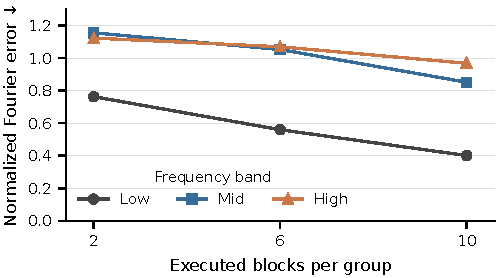
\includegraphics[width=\columnwidth]{figures/motivation/depth_frequency_v29.pdf}
\caption{Frequency-domain errors for different execution prefixes of one trained privileged network, averaged over ten fixed Urban100 images. Each curve corresponds to one radial frequency band; lower is better. This probe changes the executed blocks while retaining the trained condition updates and reconstruction head.}
\label{fig:supp_depth_frequency}
\end{figure}

\begin{figure}[!t]
\centering
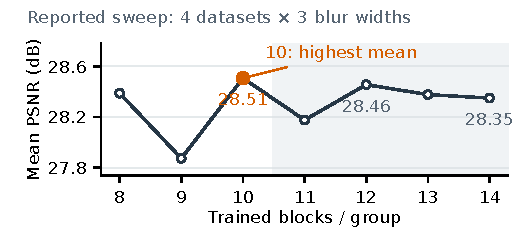
\includegraphics[width=\columnwidth]{figures/motivation/depth_sweep_diagnostic_20261029.pdf}
\caption{Historical architectural sweep: equal-weight mean over four datasets and three blur widths. The reported 8--14-block sweep also appears, with the updated twelve-block aggregate, in main Fig.~\ref{main-fig:motivation}(a) and is distinct from the fixed-teacher Fourier prefixes. Ten blocks have the highest reported mean, not a universal depth optimum.}
\label{fig:supp_depth_sweep_visual}
\end{figure}

Figure~\ref{fig:supp_depth_sweep_visual} gives the complete historical depth curve also used in main Fig.~\ref{main-fig:motivation}(a). These values come from the original reported table; checkpoint identities and training conditions for the complete sweep have not been independently reconciled. In the historical architectural sweep, 8 through 14 blocks yield overall means of 28.39, 27.87, 28.51, 28.18, 28.46, 28.38, and 28.35~dB. The twelve-block aggregate in the main figure was subsequently corrected to 28.42~dB; the archived per-condition values shown here are retained pending reconciliation. The independent depth retest gives a separate strict-load retest of teachers with 10, 12, and 14 blocks at a teacher checkpoint, each with its own PCA. The fixed indices 50--99 of Urban100 and B100 give a six-condition mean advantage of 0.117~dB for twelve over ten blocks, while fourteen is worse in every condition. The ten-block run used one GPU and batch 64; deeper runs used four GPUs, batch 16, and microbatch 8. These differences preclude a depth-only causal interpretation. Ten is the benchmark reference, not a universal or independently validation-selected optimum.


\begin{figure}[!t]
\centering
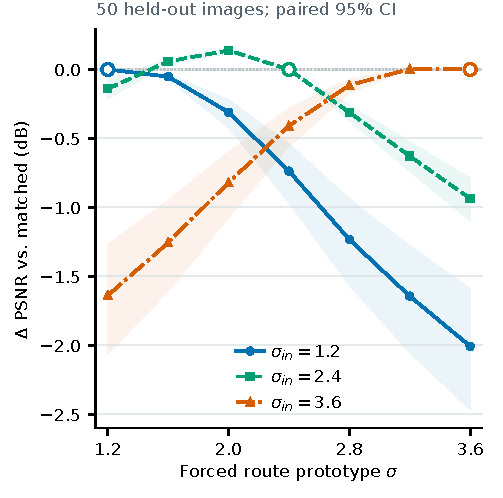
\includegraphics[width=\columnwidth]{figures/motivation/route_response_diagnostic_20261029.pdf}
\caption{Held-out response to residual-weight substitution. Curves indicate input blur widths; the horizontal axis gives the replacement prototype width and the vertical axis the PSNR change from matched weights. Shading shows paired image-bootstrap 95\% intervals. Prototypes use the first 50 Urban100 images and evaluation the remaining 50. All group corrections and the reconstruction head stay fixed; only weights change. This tests composition sensitivity, not an independent training gain from dynamic weights.}
\label{fig:supp_route_response}
\end{figure}

Figure~\ref{fig:supp_route_response} retains the quantitative route response moved from the main motivation figure. For the route-substitution visualization, the first 50 images estimate each blur-width prototype and the remaining 50 evaluate it. Across seven widths, matched prototypes exceed mismatched prototypes by 0.530~dB on Urban100 and 0.410~dB on B100 on average. Nevertheless, 9/42 and 3/42 mismatches improve PSNR, respectively. These fixed-network results diagnose sensitivity; Table~\ref{tab:supp_uniform_training} remains the relevant retraining control.

\section{Degradations and Inference Cost}
\label{sec:supp_efficiency}
\subsection{Anisotropic Blur and Noise}
The separately trained anisotropic model samples principal-axis standard deviations in $[0.2,4]$, orientation in $[0,\pi)$, and Gaussian noise standard deviation in $[0,25]$ on the 8-bit scale. Squared axis values form covariance eigenvalues. Main Table~\ref{main-tab:anisotropic} includes the complete nine-kernel B100 comparison from LightBSR Setting~2, with baseline numbers from its Table~4. The mean margins over official LightBSR are 0.018/0.016~dB at noise 5/10: 15 conditions favor DEDBSR, two tie, and one favors LightBSR. These cross-paper differences do not establish significance or zero-shot robustness.


\subsection{Operation Counts and Runtime}
\begin{table}[t]
\caption{Mechanism-level conditions and inference cost. THOP uses $180\times320$ LR input and one MAC per operation; the $64\times64$ row uses PyTorch's two-FLOP-per-MAC convention. DEDBSR transfer conditions share one forward graph.}
\label{tab:supp_efficiency_conditions}
\centering\scriptsize
\setlength{\tabcolsep}{1.8pt}
\renewcommand{\arraystretch}{0.94}
\resizebox{\columnwidth}{!}{%
\begin{tabular}{lrrrl}
\toprule
Condition & Params. & Cost & Mean/U100 SSIM & Interpretation\\
\midrule
\multicolumn{5}{l}{\textit{DEDBSR transfer and routing conditions}}\\
Full adaptive & 4.1M & 245.5907 G & .7903/.7796 & reference\\
GT-only init. & 4.1M & 245.5907 G & .7905/.7809 & no output KD\\
Frozen inherited & 4.1M & 245.5907 G & .7851/.7654 & no adaptation\\
Uniform routing (two states) & 4.1M & 245.5907 G & .7903--.7905/.7796--.7803 & fixed weights\\
\midrule
\multicolumn{5}{l}{\textit{Cross-model profiling references}}\\
CdCL-S & 2.9M & 130.8508 G & --/-- & no matched SSIM\\
CdCL-L & 5.9M & 201.68 G & --/-- & reported profile\\
LightBSR & 3.26M & 181.1965 G & --/-- & architecture only\\
DEDBSR student, $64^2$ & 4.1M & 34.9444 GF & --/-- & timing only\\
\bottomrule
\end{tabular}}
\end{table}


We profile complete inference with THOP 0.1.1 at batch one, using $180\times320$ RGB LR inputs and $\times4$ outputs. DEDBSR requires 245.5907~G operations; CdCL-S and LightBSR require 130.8508 and 181.1965~G. Convolution and linear MACs count as one operation; pooling and BatchNorm follow THOP defaults. Counts are executed profiles, not area extrapolations.

DEDBSR and official CdCL-S weights are loaded; LightBSR uses its published architecture without trained weights and therefore supplies complexity only. Its implementation has 3,259,971 parameters versus the paper's rounded 3.1M, while its reported 206.16~G uses $256\times256$ input. CdCL-S's reported 91.68~G differs from our released-implementation profile. These mixed sources do not establish a unified efficiency ranking.

A separate $64\times64$ LR test of the archived student implementation uses RTX 4090 D, FP32, batch one, 20 warm-ups, and 100 CUDA-event forwards: 49.13~ms mean latency and 189.6~MB peak memory. PyTorch counts 34.9444~GFLOPs at this size (two FLOPs per MAC), so this is distinct from the THOP profile. All profiles exclude training costs. Parameter entries retain the reported model-size convention; the archived runtime and operation profiles do not independently validate that parameter count.
\end{document}
